\documentclass[12pt,a4paper,ngerman]{report}
\usepackage{babel}
%\usepackage{natbib}
\usepackage{url}
%\usepackage[left=2cm, right=1.5cm, top=2cm, bottom=2cm]{geometry}
%\usepackage[ansinew]{inputenc}
\usepackage{amsmath}
\usepackage{nicefrac} % macht schöne Brüche mit querstrich mit \nicefrac{1}{2}
\usepackage{graphicx}
%\graphicspath{}
\usepackage{titlesec}% um chapterüberschriften anzupassen.
\titleformat{\chapter}{\normalfont\huge\bf}{\thechapter.}{20pt}{\huge\bf}
\usepackage{parskip}
\usepackage{fancyhdr}
\usepackage{amsfonts}
\usepackage{float}
\usepackage{caption}
\usepackage{subcaption} % for \begin{subfigure}
	
\usepackage{csquotes} % mit \enquote{blabla} tolle anfürungsstriche erstellen
%\usepackage{physics} %lässt mich \bra und \ket benuzen %im konflict mit siunitx

\usepackage{pgfplots} %für plots
\pgfplotsset{compat=newest}

\usepackage{varioref} % macht mit \vref{} viel bessere referenzen
\usepackage{hyperref} % macht klickbare referenzen

\usepackage{xcolor, soul} %mit \hl{} kann man toll Sachen hervorheben.
\newcommand{\highlight}[1]{%
	\colorbox{yellow!50}{$\displaystyle#1$}} % mit \highlight{} kann man sogar in Gleichungen hervorheben

\usepackage{vmargin}
\usepackage[section]{placeins}
\usepackage{capt-of}
\usepackage{enumitem}
\usepackage{multirow}
\usepackage{blindtext}
\usepackage[version=4]{mhchem} % um Chemische Elementsymbole zu benutzen: \ce{H20}

\usepackage{pdfpages} % um PDFs einzufügen

%spread to latex:
\usepackage{booktabs, multirow} % for borders and merged ranges
\usepackage{changepage,threeparttable} % for wide tables

\providecommand{\e}[1]{\ensuremath{\cdot 10^{#1}}}
\providecommand{\fehlt}{\textcolor{red}{\emph{Fehlt!\dots}}}

\usepackage{siunitx}
\sisetup{
	separate-uncertainty = true,
	%per-mode = fraction,
	%per-mode = symbol
}
\DeclareSIUnit\bar{bar}
\DeclareSIUnit\atomicmassunit{u}
\usepackage{isotope}


\setmarginsrb{3 cm}{2.5 cm}{3 cm}{2.5 cm}{1 cm}{1.5 cm}{1 cm}{1.5 cm}
\title{Myonenzerfall}			%%%%%%%%%%
% Title


\author{Frederik Uhlemann, F. Adamczyk}
% Author
\date{\today}
% Date

\makeatletter
\let\thetitle\@title
\let\theauthor\@author
\let\thedate\@date
\makeatother

\pagestyle{fancy}
\fancyhf{}
\rhead{\theauthor}
\lhead{Myonenzerfall}
\cfoot{\thepage}
%%%%%%%%%%%%%%%%%%%%%%%%%%%%%%%%%%%%%%%%%%%%
\begin{document}
		
	%%%%%%%%%%%%%%%%%%%%%%%%%%%%%%%%%%%%%%%%%%%%%%%%%%%%%%%%%%%%%%%%%%%%%%%%%%%%%%%%%%%%%%%%%
	
	\begin{titlepage}
		\centering
		\vspace*{0.5 cm}
		% \begin{large} Justus-Liebig-Universität\\ Gießen \end{large}
		
\includegraphics[width = 0.6 \textwidth]{JLU_Giessen-Logo}	%University Logo
		\\[2.0 cm]
		% \begin{center}    \textsc{\Large Justus - Liebig - Universität}\\{Giessen}\\[0.8cm]	\end{center}% University Name
		Versuch 5 des\\
		\textsc{\Large  Fortgeschrittenen-Praktikums}\\ [0.3 cm]				% Course Code
		\rule{\linewidth}{0.2 mm} \\[0.4 cm]
		{ \huge \bfseries \thetitle}\\%%% TITEL HERE
		\rule{\linewidth}{0.2 mm}\\
		Versuchstermin Freitag, 31.05.2024 \\
		~ \\
		[2.0 cm]
		
		
		\begin{minipage}{0.49\textwidth}
			\begin{flushleft}
				 \emph{Praktikumsbetreuer:}\\
				 Marvin Peter\\
				 %  Affiliation\\
				 \small{\href{mailto:marvin.peter@exp2.physik.uni-giessen.de}{marvin.peter@exp2.physik.uni-giessen.de}}
			\end{flushleft}
		\end{minipage}~
		\begin{minipage}{0.49\textwidth}
			\begin{flushright}
				\emph{Protokoll von:} \\
				
				\large{Frederik Uhlemann}\\
				\small{\href{mailto:frederik-vincent.uhlemann@physik.uni-giessen.de}{frederik-vincent.uhlemann@physik.uni-giessen.de}\\~\\
					%Matrikel Nr.: \:  \\[0.5cm]
					%\href{mailto:}{}
				}
				\large{Florian Adamczyk} \\
				\small{\href{mailto:florian.marius.adamczyk@physik.uni-giessen.de}{florian.marius.adamczyk@physik.uni-giessen.de}\\
					%Matrikel Nr.: \: 8105234}
			}
		\end{flushright}
	\end{minipage}
	
	\end{titlepage}
	
%%%%%%%%%%%%%%%%%%%%%%%%%%%%%%%%%%%%%%%%%%%%%%%%%%%%%%%%%%%%%%%%%%%%%%%%%%%%%%%%%%%%%%%%%
\setcounter{secnumdepth}{3}
\setcounter{tocdepth}{4}
\tableofcontents
%\newpage

%%%%%%%%%%%%%%%%%%%%%%%%%%%%%%%%%%%%%%%%%%%%%%%%%%%%%%%%%%%%%%%%%%%%%%%%%%%%%%%%%%%%%%%%%
%\renewcommand{\thesection}{\arabic{section}} %lässt in den subsections die erste zahl von darüberliegenden chapter weg.

%\pagebreak
	
%\setcounter{chapter}{-1}
\chapter*{Einleitung}
	\addcontentsline{toc}{chapter}{Einleitung}
	Das Myon, ein Teilchen der Leptonenfamilie wie das Elektron, ist aufgrund seiner kurzen Lebensdauer und seiner Fähigkeit, die Erdoberfläche zu erreichen, besonders interessant für die Hochenergiephysik. Mit einer Masse, die etwa \num{200} Mal größer ist als die des Elektrons, bietet das Myon spannende Möglichkeiten für physikalische Untersuchungen. Ziel des Experiments ist es, die Lebensdauer dieser kosmischen Myonen zu bestimmen. Diese Myonen stammen aus der kosmischen Strahlung, die permanent auf die Erde trifft. Um die Lebensdauer zu messen, wird zunächst eine Energieeichung durchgeführt, bei der das Energiespektrum einer \ce{^60Co}"~Quelle aufgenommen wird. Danach wird die Energiedeposition minimal ionisierender Myonen in einem \ce{NaI}"~Szintillationsdetektor ermittelt. Schließlich wird der endgültige Versuchsaufbau eingerichtet, eine Zeiteichung vorgenommen und eine einwöchige Datenaufnahme gestartet.


	% notiz an mich: mit "~ bewirke ich einen geschützten bindestrich an dem nicht getrennt werden darf.
	% nur eine ~ macht ein geschütztes (normales) Leerzeichen. \, macht ein halbes geschütztes Leerzeichen.

\chapter{Theorie}
	\section{Myonen}
	Das Myon, ein grundlegendes Teilchen der Leptonenfamilie, weist eine negative Elementarladung und eine Masse von etwa \qty{105,658}{\mega\electronvolt\per c\squared} auf, was etwa dem 200"~fachen der Elektronenmasse entspricht. Aufgrund seiner Natur als Fermion besitzt es einen Spin von $\nicefrac{1}{2}$ und unterliegt sowohl der elektromagnetischen als auch der schwachen Wechselwirkung, zeigt jedoch keine starke Wechselwirkung. Das Antiteilchen des Myons ist das Antimyon, welches dieselbe Masse und Spin, jedoch eine entgegengesetzte Ladung aufweist. \\

	Myonen entstehen hauptsächlich aus der kosmischen Strahlung, die durch Wechselwirkung hochenergetischer Protonen mit den Gasmolekülen der Erdatmosphäre erzeugt wird. Diese Kollisionen führen zur Entstehung von Pionen, die anschließend in Myonen und Myon"~Neutrinos zerfallen. Aufgrund ihrer kurzen Lebensdauer von etwa \qty{2,2}{\micro\second} im Ruhesystem stellt sich die Frage, wie sie die Erdoberfläche erreichen können. Hier kommt die spezielle Relativitätstheorie ins Spiel: Durch die Zeitdilatation wird die Lebensdauer der Myonen relativ zur Erdoberfläche verlängert, sodass sie mehrere Kilometer zurücklegen können, bevor sie zerfallen. Aus Inertialsystem der Myonen betrachtet erfahren sie aufgrund der Lorentz-Kontraktion eine Längenverkürzung in Bewegungsrichtung, was ihre Wahrscheinlichkeit erhöht, die Erdatmosphäre zu durchdringen. \\
	
	In Experimenten wird die Zerfallszeit der Myonen gemessen, indem die Produkte ihres Zerfalls, ein Elektron und ein Antielektron-Neutrino, detektiert werden. Für diese Messungen werden \ce{NaI}"~Szintillationsdetektoren eingesetzt, die die Energiedeposition der minimal ionisierenden Myonen bestimmen. 

		\begin{figure}[ht]
		\centering
		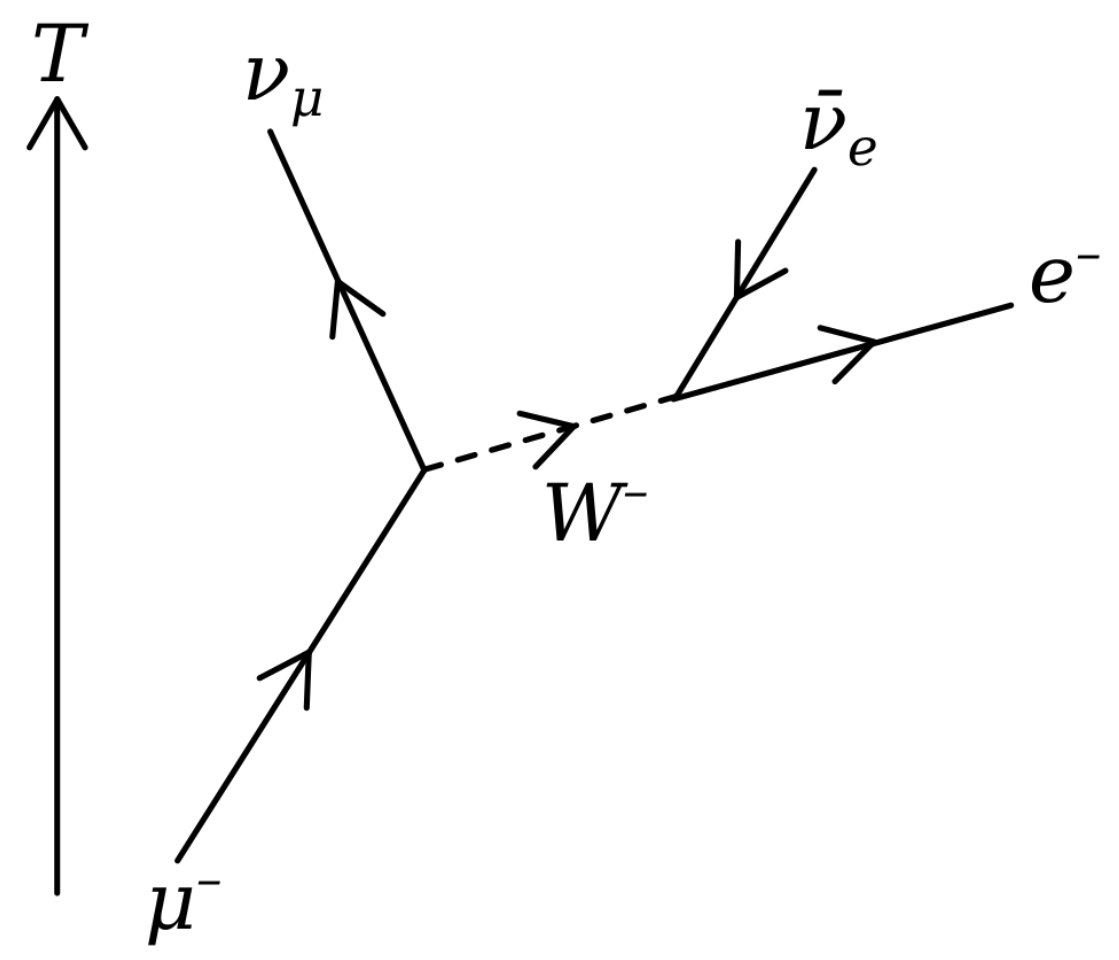
\includegraphics[width=.7\textwidth]{Bilder/Feynman_Myon}		
		\caption{Feynman"~Diagramm des Myonenzerfalls}
		\label{fig:Feynman_Myon}
	\end{figure}
	
	Die zu Feynman Diagramm (siehe Abb. \ref{fig:Feynman_Myon}) gehörende Zerfallsreaktion lautet:
	\[\mu^{-}_{m} \rightarrow e^{-} + \nu_e + \nu_{\mu} \]
	
	Es kann auch zusätzlich ein Photon emittiert werden:
	\[\mu^{-}_{m} \rightarrow e^{-} + \nu_e + \nu_{\mu} + \gamma \]
	
	Negative Myonen sind instabile Elementarteilchen, die sowohl im Vakuum als auch in Materie zerfallen können. Im Gegensatz zu ihrem Verhalten im Vakuum haben negative Myonen in Materie einen zusätzlichen Zerfallskanal.
	
	Ein Myon kann mit einem Atomkern wechselwirken und ein sogenanntes “myonisches Atom” bilden. Da Myonen und Elektronen im Wesentlichen nur durch ihre Masse unterschieden werden, können sie sich auch an Atomkerne binden. Aufgrund ihrer deutlich höheren Masse sind Myonen jedoch viel stärker an den Kern gebunden. Dadurch haben sie eine etwa siebenfach höhere Wahrscheinlichkeit, sich im Kernbereich aufzuhalten.
	
	Dies führt dazu, dass ein Myon in Materie analog zum Elektroneneinfang vom Kern absorbiert werden kann. Dabei wird ein Proton in ein Neutron umgewandelt, und ein Myonneutrino wird emittiert. Dieser zusätzliche Zerfallskanal beeinflusst die experimentell bestimmte durchschnittliche Lebensdauer von negativen Myonen in Materie, die kürzer ist als im Vakuum.

	\section{Messung gestoppter Myonen} \label{ch:Mess}
		Das Zerfallsgesetz von Myonen lautet:
		\[\frac{dN}{dt}= -\lambda N(t)\]
		und die allgemeine Lösung dieses Gesetzes ist:
		\[N(t) = N_0 \cdot e^{-lambda t}\]
		
		Die mittlere Lebensdauer ist die Zeit $\tau$, nch dem vorraussichtlich noch $\nicefrac{1}{e}$ Teilchen der Anfangsmenge $N_0$ übrig sind. \\
		Setzt man das in das Zerfallsgesetz ein erhält man:
		\[T_{\nicefrac{1}{2}} = \frac{\ln(2)}{\lambda} = \tau \cdot \ln(2) \].
		
		Um Myonen zu detektieren, werden sie in einem Natriumiodid (NaI)-Detektor eingefangen, und die Zerfallsprodukte werden gemessen. Die Grenzenergie, bei der Myonen in einem 10 cm dicken NaI-Material gestoppt werden können, lässt sich aus Abbildung 7 in der Anleitung  \cite{Anleitung} ablesen.
		
		Die Dichte des NaI-Materials beträgt $\rho = 3,67 g/cm^3$, was einer Dicke von l = 10 cm entspricht ($\rho_l = 36,7 g/cm^2$). Myonen, deren Reichweite (durch ihre Energie bestimmt) über diesem Wert liegt, werden nicht mehr gestoppt. Diese Reichweite wird als Grenzenergie definiert. Abbildung 7 zeigt, dass diese Reichweite für eine Grenzenergie von etwa $E_max  \qty{90}{\mega\electronvolt} \text{ bis } \qty{100}{\mega\electronvolt}$ erreicht wird.
		
		Der Begriff \glqq minimal ionisierend\grqq ~bezieht sich auf Teilchen, die genau den Impuls aufweisen, bei dem die Änderung der übertragenen Energie pro zurückgelegter Strecke, minimal ist. Die Analyse von Abbildung 6 in der Anleitung verdeutlicht, dass dieses Minimum im Bereich von 200 GeV/c bis 300 GeV/c liegt und einen Wert von \qty{1,2}{\mega \electronvolt\per\gram} bis \qty{1,3}{\mega \electronvolt\per\gram} erreicht.
		

\chapter{Aufbau und Messprinzip}
	\section{Szintillator und Photomultiplier}
	In diesem Experiment werden die kosmischen Myonen wie im vorangestellten Kapitel \ref{ch:Mess} mittels eines Szintillatonsdetektors gemessen. Wie dadurch ein Messbares Signal entsteht, soll im folgenden kurz erläutert werden.\\
	Wenn geladene Teilchen, wie das Myon durch den Natriumiodit Kristall fliegen, regen diese die Elektronen in den Hüllen der Atome im Kristall an und heben sie damit auf ein höheres Energieniveau. Im Kristall werden somit Elektronen und Löcher freigesetzt, wenn diese sofort rekombinieren würden, würde ein hochenergetisches Photon entstehen, dieses hätte die gleiche Abregunsenergie wie die Anregungsenergie von $NaI$, damit kann es nicht im Szintillator gemessen werden.\\
	Die Lösung ist, dass der Kristall dotiert wird, bei $NaI$ typischerweise mit Thallium. Dadurch werden zusätzliche Energieniveaus in dem Kristall hinzugefügt. So wandern die Elektronen und Löcher über diese Niveaus zu den sogenannten Lumineszenzzentren. Dieses angeregte Zentrum, regt sich über die Aussendung von optischen Photonen habt. Diese haben nun deutliche geringere Energien, im sichtbaren oder UV-Bereich und können durch den Kristall zum Photomultiplier wandern.\\
	Wenn ein optisches Photon auf die Photokathode des Photomultipliers trifft, kann durch den Photoeffekt ein Photoelektron entstehen. Dieser Prozess ist abhängig von der Quanteneffizienz des Anoden Materials, dass bedeutet nicht jedes Photon erzeugt ein Photoelektron. Falls ein Elektron entstandenen ist, wird es auf ein Elektrode gelenkt, trifft es auf dieser sogenannten Dynode, schlägt es weitere Elektronen heraus. Diese treffen erneut auf eine weitere Dynode, der Prozess wiederholt sich einige Male. So einstehen durch ein Schneeballsystem viele Elektronen, die so einstehende Ladung kann gemessen werden.  
	
	 
	\section{elektronische Signalverabeitung}
	\subsection{Messprinzip der Energiemessung}\label{ch:EnergieMessung}
	In der ersten Messung wird das Gammaspektrum einer Cobalt-60 Quelle aufgezeichnet. Der verwendete Messaufbau ist in der Abbildung \ref{img:EnergieAufbau} schematisch dargestellt. Wie im vorherigen Kapitel beschrieben, gibt der Photomultiplier ein Signal aus, dieses ist negativ. Der Hauptverstärker invertiert das Signal und gibt es dann dem Analog-Digital-Umwandler. Mit diesem kann der Computer ein Histogramm speichern. Der verwendete ADC hat 8064 Kanäle.
	\begin{figure}[ht]
		\centering
		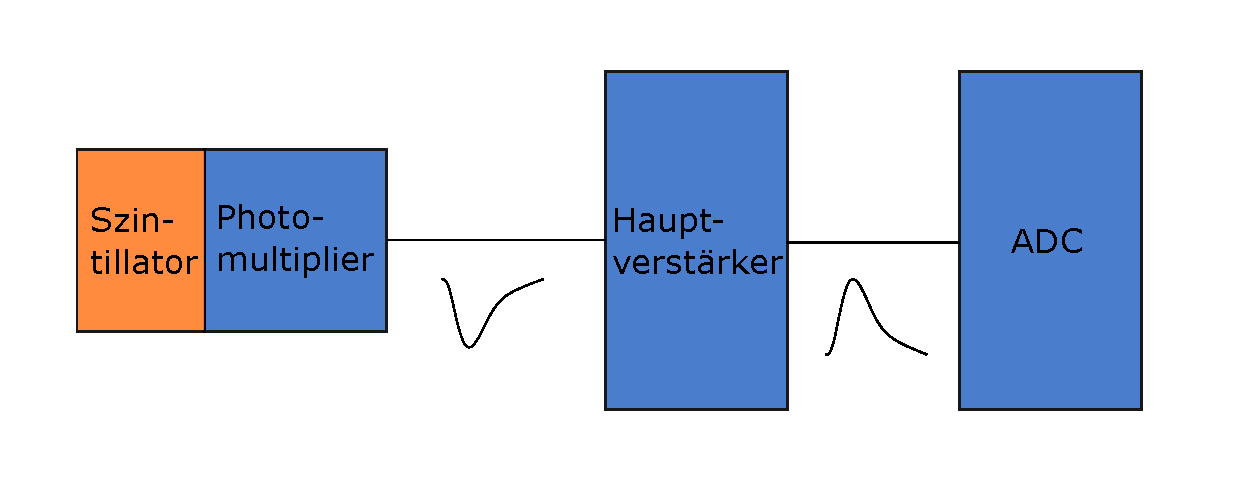
\includegraphics[width=\textwidth]{Bilder/Energiemessung.pdf}		
		\caption{Messprinzip der Energiemessung, simpler Aufbau aus Szintillator mit PMT, Verstärker und ADC}
		\label{img:EnergieAufbau}
	\end{figure}
	\subsection{Messprinzip der Zeitmessung}
	Das Prinzip der Zeitmessung besteht darin, die Myonen im Szintillator vollständig zu stoppen und dann die Zeit bis zu ihrem Zerfall zu bestimmen. Durch die Zeitdifferenz kann die Lebensdauer bestimmt werden. Wenn ein Signal detektiert wird, ist nicht klar ob es ein Start oder Stopp Signal eines Myons war. Deshalb gilt jedes Signal sowohl als Start und Stopp gleichzeitig. In der Abbildung \ref{img:ZeitEinfach} ist der Aufbau zu sehen.
	\begin{figure}[ht]
		\centering
		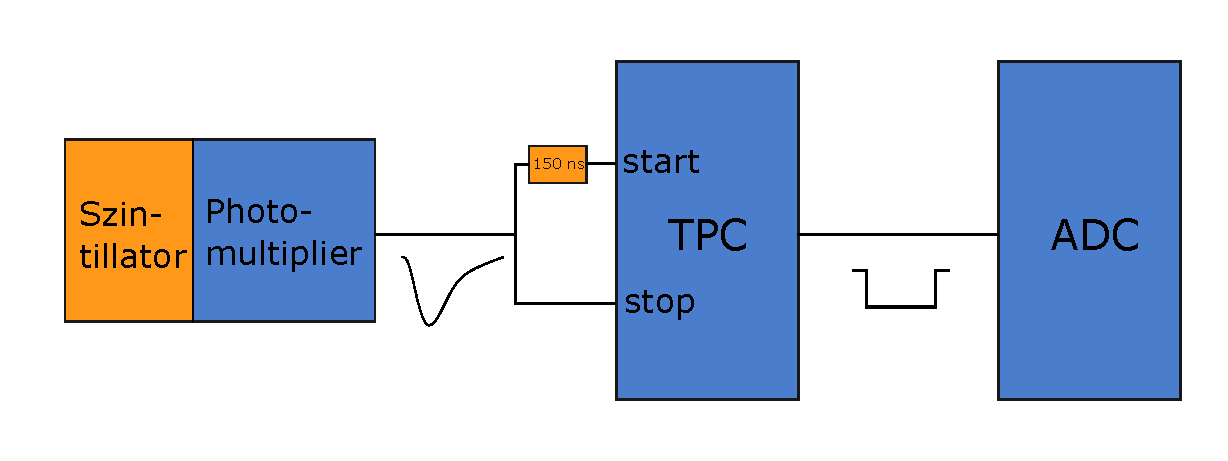
\includegraphics[width=\textwidth]{Bilder/ZeitmessungEinfach.pdf}		
		\caption{Schematischer Aufbau der Zeitmessung, jedes Signal wird als Start und Stop Signal verwendet, wobei dem Start ein Delay hinzugefügt wird }
		\label{img:ZeitEinfach}
	\end{figure}
	Durch eine Verzögerung von \SI{150}{\nano \second}, kommt das Startsignal nach dem Stoppsignal im Time to Pulse Height Converter (TPC) an. Der TPC liefert ein Signal welches proportional zur Zeitdifferenz zwischen Start und Stopp ist. Mit Hilfe dieser Differenz, kann die Lebensdauer ermittelt werden.\\
	\begin{figure}[ht]
		\centering
		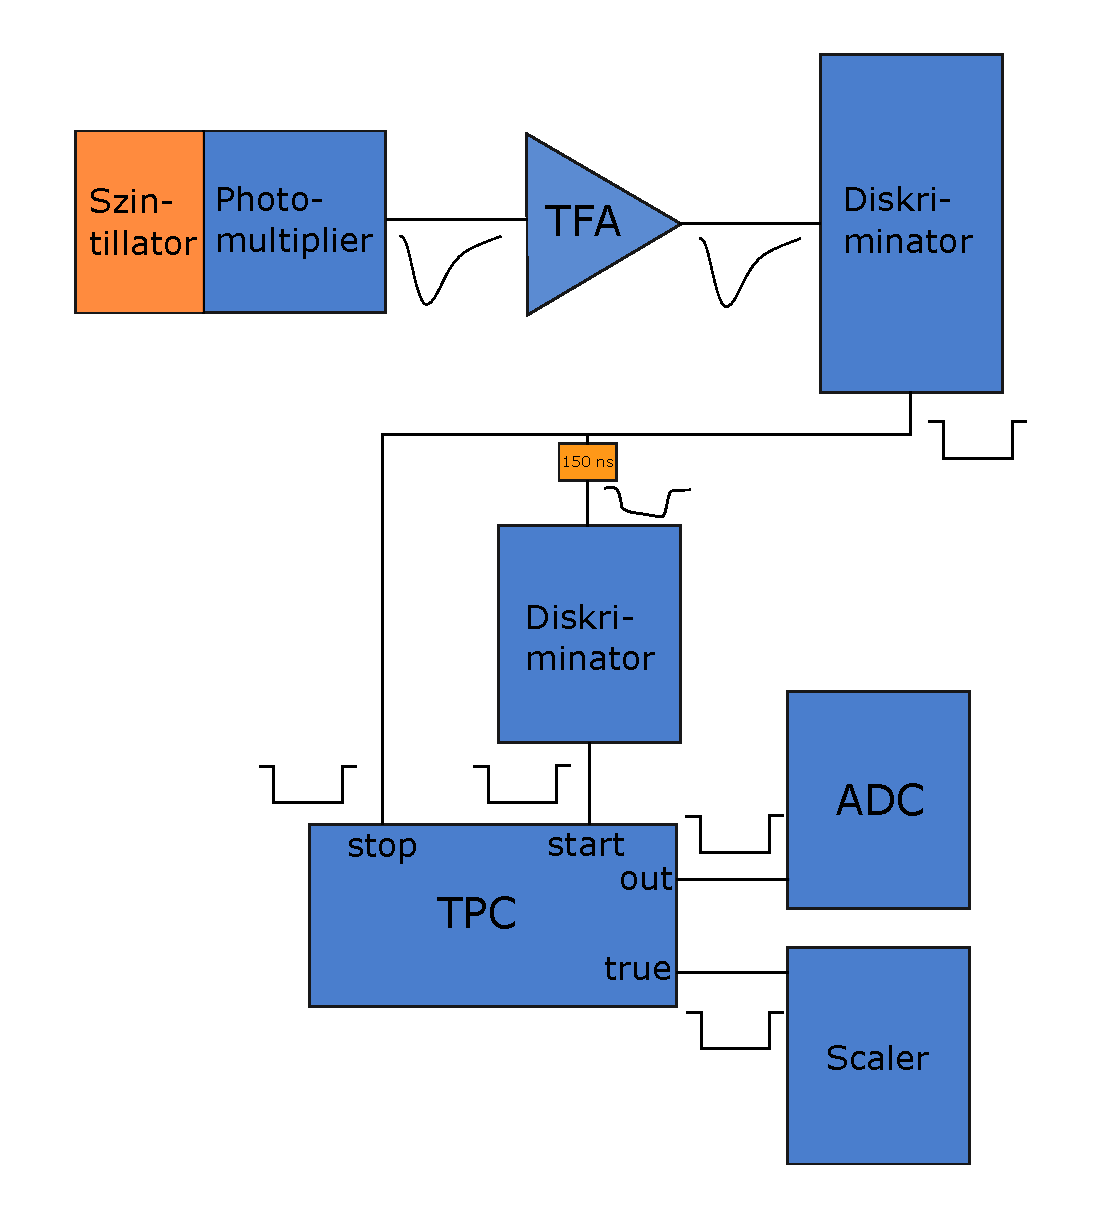
\includegraphics[width=\textwidth]{Bilder/ZeitmessungKomplex.pdf}		
		\caption{Vollständiger schematischer Messaufbau}
		\label{img:ZeitmessungKomplex}
	\end{figure}
	Der vollständige Messaufbau mit allen Komponenten ist in \ref{img:ZeitmessungKomplex} abgebildet, im Gegensatz zum prinzipiellen Aufbau aus Abbildung \ref{img:ZeitEinfach}, sind elektronische Komponenten hinzugekommen. Wie zum Beispiel ein Timing Filter Amplifier (TFA), dieser Verstärkt das Signal, ohne es stark zu verzerren. Der erste Diskriminator soll den natürlichen radioaktiven Untergrund abschneiden. Das um \SI{150}{\nano \second} Verzögerte Signal, wird in einem weiteren Diskriminator wieder zum guten Rechtecksignal verarbeitet. weil es durch die lange Kabelführung im Delay verzerrt wird. Der TPC welcher die Zeitdifferenz von Start uns Stopp ermittelt, gibt zusätzlich zu seiner grundsätzlichen Arbeitsweise, noch ein logisches Signal bei jedem "Start" aus. Dieses wird an einen Scaler gegeben, welcher einfach die Ereignisse zählt.
	
	
	


\chapter{Auswertung der Daten}


	\section{Energieeichung}
		Zu aller erst soll sich mit dem Versuchsaufbau vertraut gemacht werden. Hierfür wird das Energiespektrum einer \isotope[60]{Co}-Probe aufgenommen. Der verwendete Messaufbau wurde im Kapitel \ref{ch:EnergieMessung} erläutert. Das ermittelte Spektrum ist in Abbildung \ref{img:GammaCo60} dargestellt, das Spektrum ist zweimal abgebildet, wobei das untere mit logarithmischer y-Achse dargestellt ist.\\
		Es sind die beiden typischen Gammapeaks bei \SI{1173.2}{\kilo \eV} und \SI{1332.5}{\kilo \eV} erkennbar, zusätzlich ist gerade in der logarithmischen Darstellung, gut der Summenpeak dieser beiden zu erkennen. 
		\begin{figure}[ht]
			\centering
			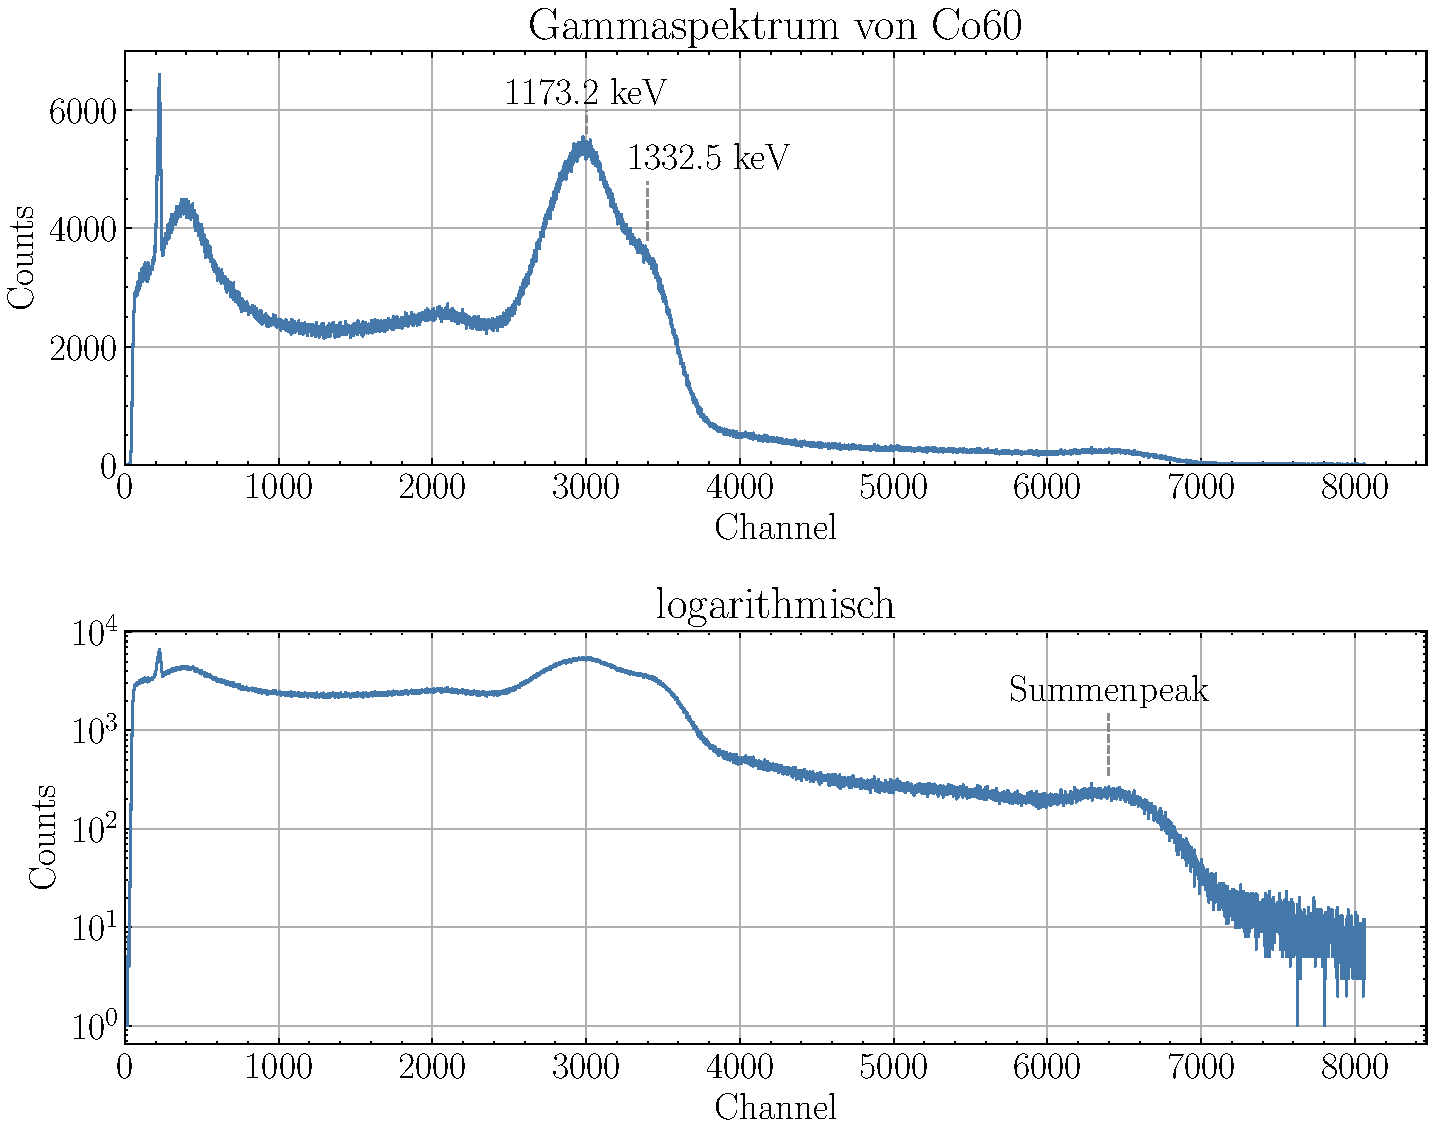
\includegraphics[width=\textwidth]{Bilder/GammaCo60.pdf}		
			\caption{Gammspektrum der \isotope[60]{Co}-Probe, es lassen sich die 2 Gamma Peaks erkennen, in der logarithmischen Darstellung, ist auch der Summenpeak deutlich sichtbar}
			\label{img:GammaCo60}
		\end{figure}
	Mit Hilfe der Kenntnis über die ungefähre Lage des Summenpeaks, soll der Verstärker so eingestellt werden, dass ein Energiebereich für die minimal ionisierenden
	Myonen gewählt wird, da diese das Ziel der eigentlichen Messung sind. (Energiebereichschätzung sollte erwähnt werden \fehlt)
	\begin{figure}[ht]
		\centering
		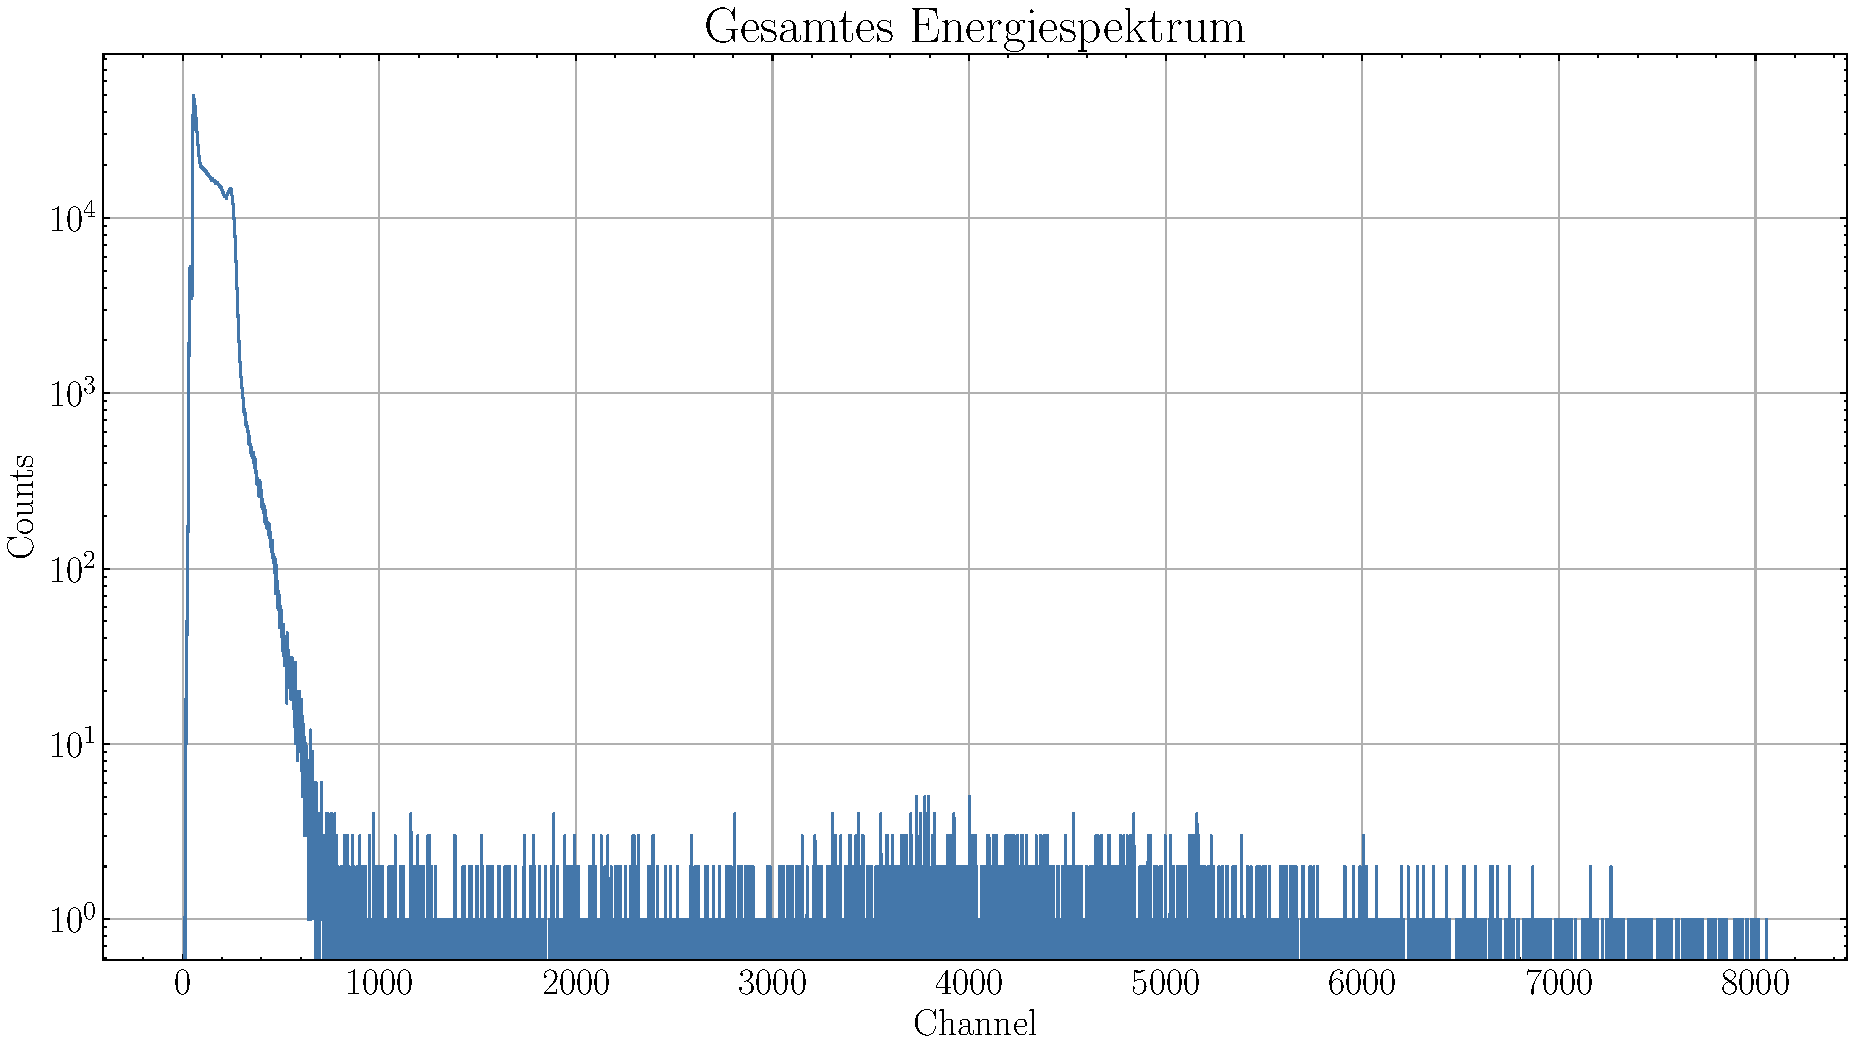
\includegraphics[width=\textwidth]{Bilder/gesamterEnBereich.pdf}		
		\caption{Gesamtes Energiespektrum, welches während der Zeitmessung verwendet wird}
		\label{img:gesamterEnBereich}
	\end{figure}
	Der gesamte Energiebereich ist in Abbildung \ref{img:gesamterEnBereich} zu erkennen, es ist erneut logarithmisch aufgetragen. Auf der linken Seite ist noch die \isotope[60]{Co}-Quelle zu erkennen. zwischen den Kanälen 3000 und 8000, befinden sich die Energieeinträge der kosmischen Myonen. Da sie eine hohe Energie besitzen und nur durch eine relativ dünne Schicht zur Ionisation fliegen, sollte ihr Energiedeposit nach Bethe-Bloch einer Landau-Verteilung entsprechen.\\
	Deshalb wurde in Abbildung \ref{img:MyonenLandau}, das Energiespektrum im entsprechendem Bereich erneut geplottet. Zudem wurden jeweils 16 Kanäle zu einem zusammengefasst, sodass nur noch 512 übrig bleiben, weil es sehr wenige Einträge pro Kanal gibt. Qualitativ wurde eine Landauverteilung an die Daten gefittet, quantiative Werte können ohne eine komplette Energieeichung nicht angegeben werden. Die Verteilung passt sich gut an die Daten, auf der linken Seite des Spektrums, sind vermutlich noch Resteffekte von radioaktiver Strahlung erkennbar. 
	\begin{figure}[ht]
		\centering
		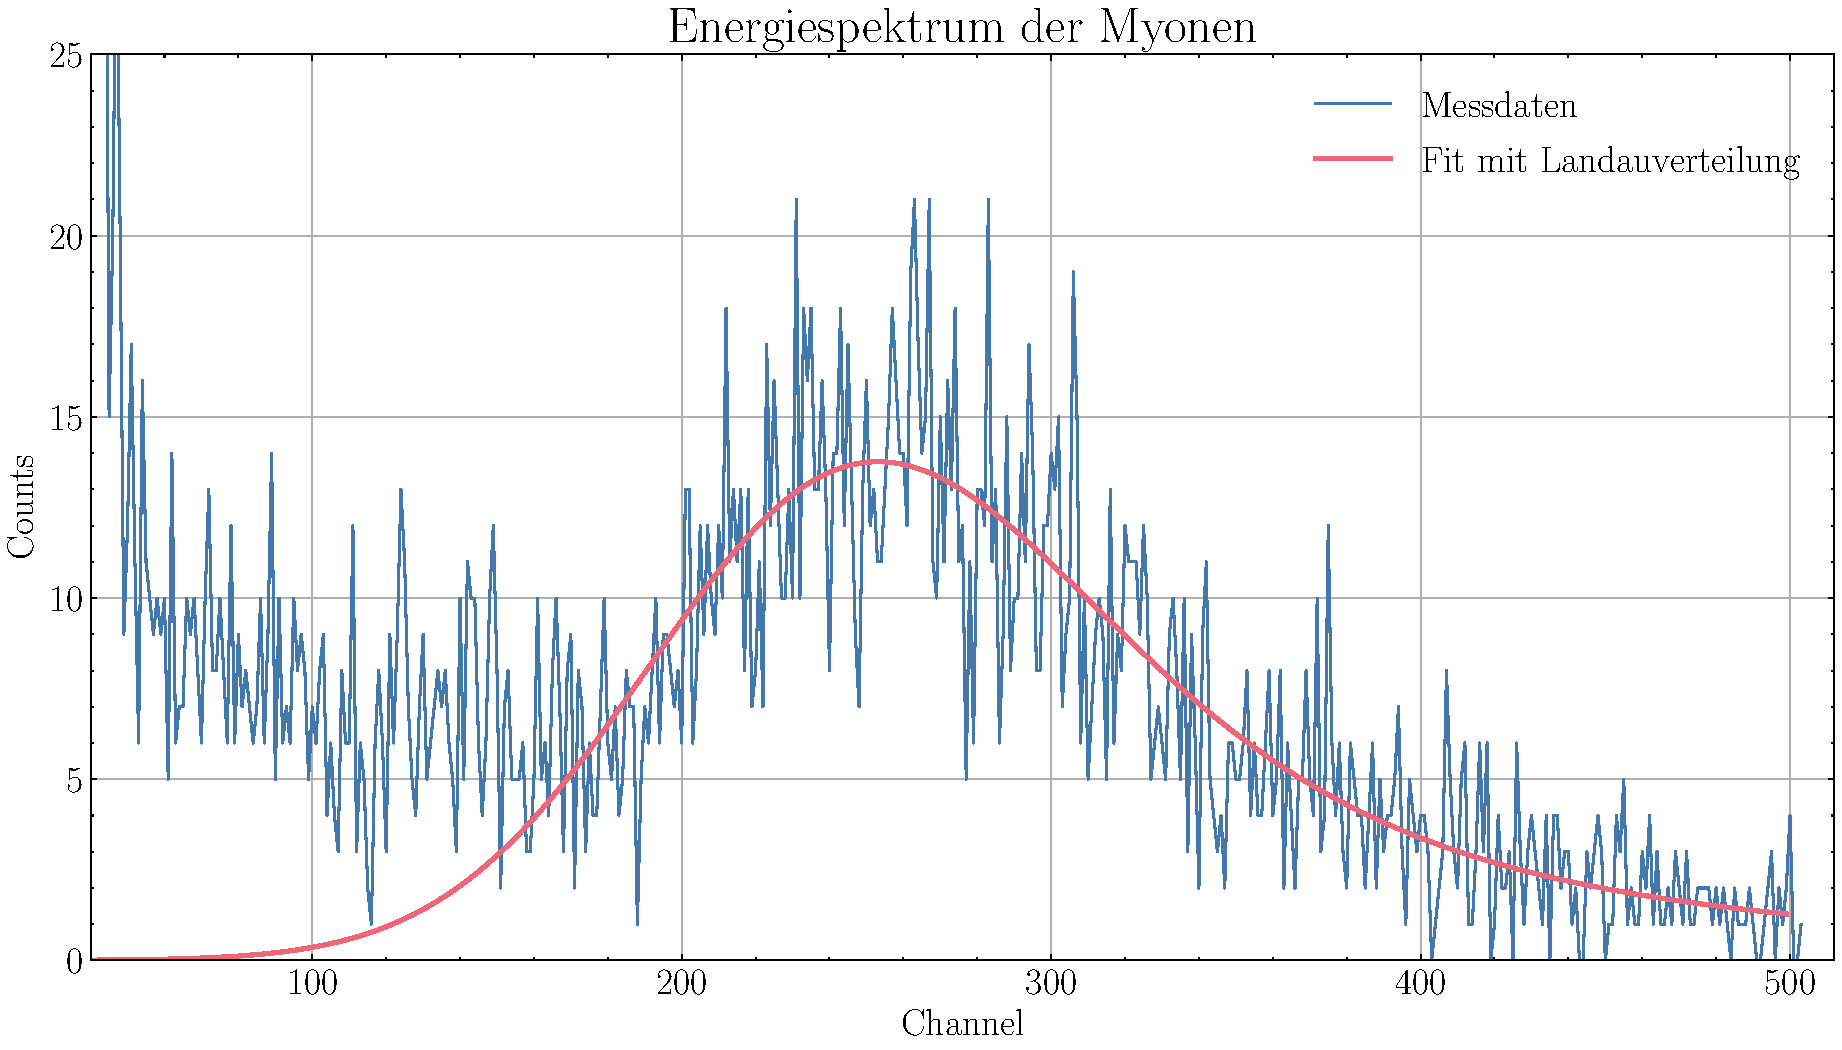
\includegraphics[width=\textwidth]{Bilder/MyonenLandau.pdf}		
		\caption{Energiedepositspektrum der kosmischen Myonen im Szintillator, mit einer qualitativer Landauverteilung}
		\label{img:MyonenLandau}
	\end{figure}
	\section{Zeiteichung}
	\begin{figure}[ht]
		\centering
		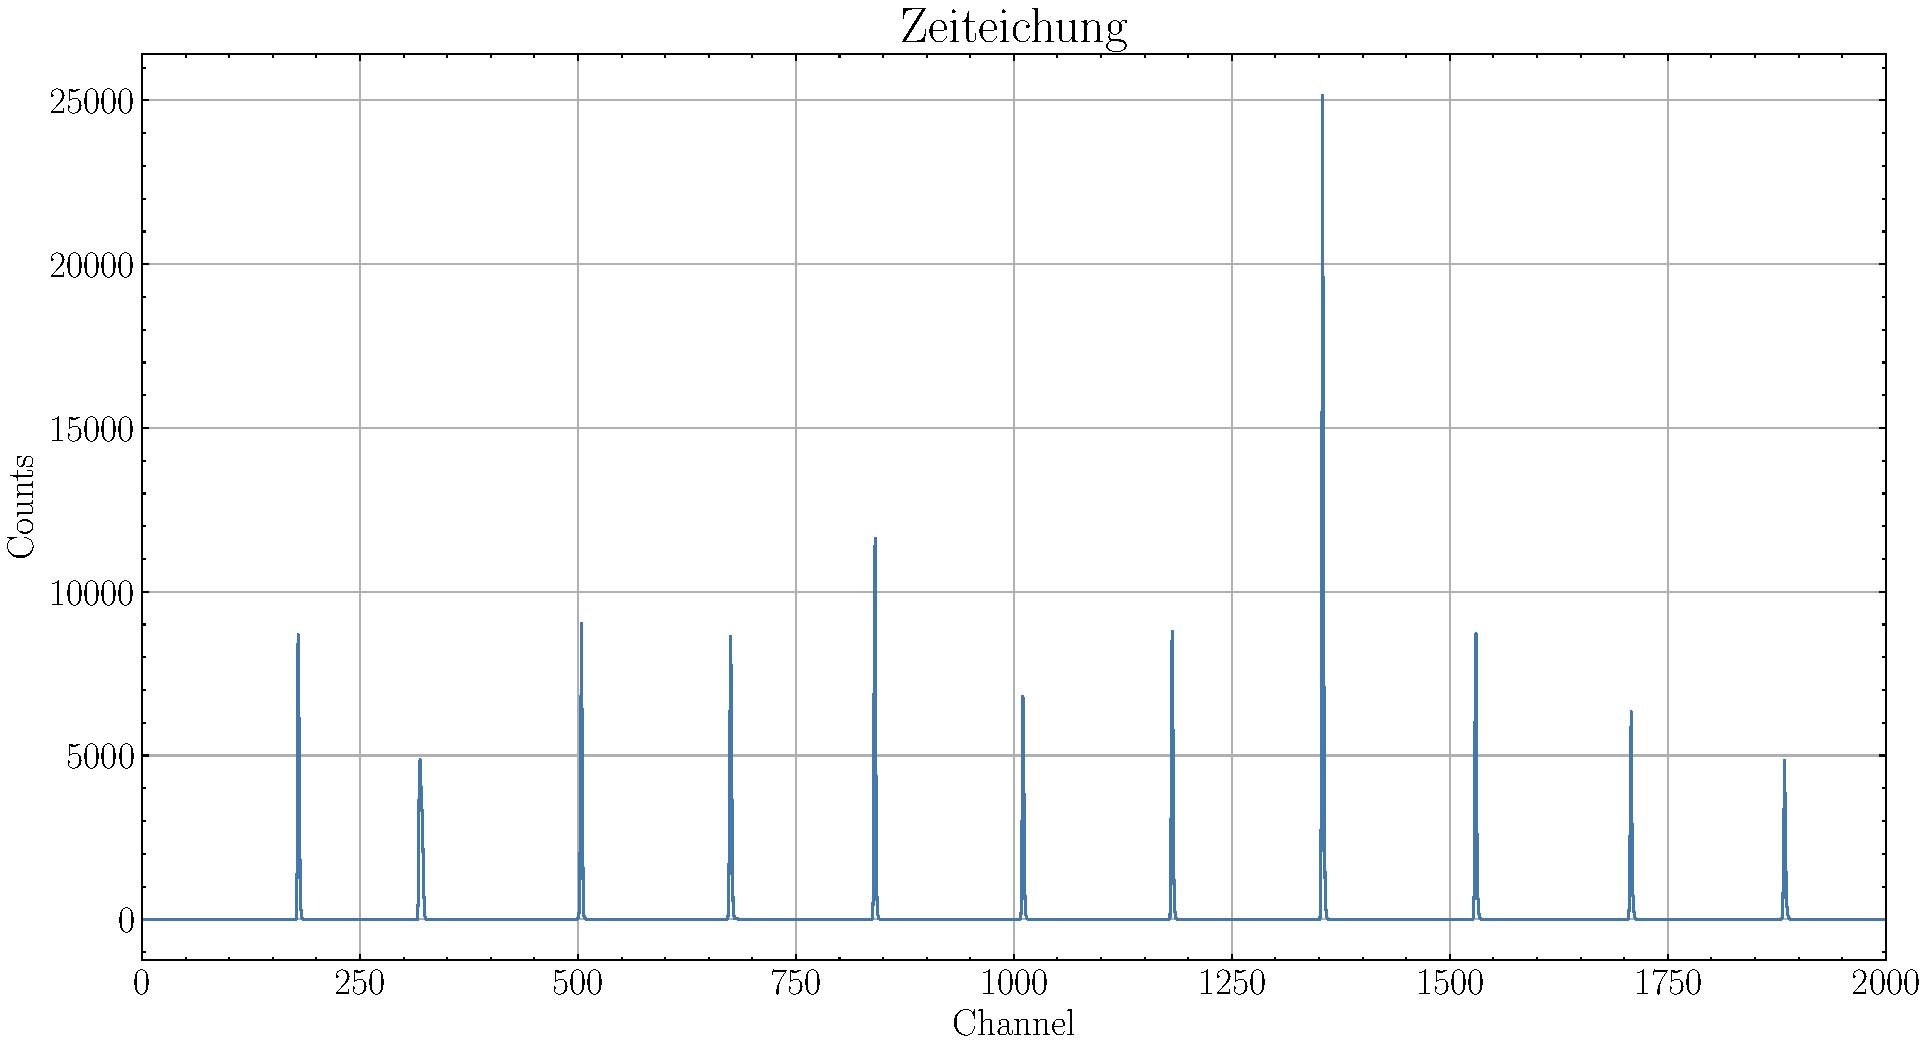
\includegraphics[width=\textwidth]{Bilder/zeitEich.pdf}		
		\caption{Spektrum der Zeiteichung, zu sehen sind die einzelnen Peaks für die jeweiligen Verzögerungen, angefangen bei \SI{300}{\nano \s} und in \SI{150}{\nano \s} Schritten bis \SI{1800}{\nano \s}}
		\label{img:zeitEich}
	\end{figure}
	Der ADC gibt Kanäle an den Computer, diese müssen mittels einer Zeiteichung in Zeitwerte [s] umgerechnet werden. Dafür werden bekannte Verzögerungen vor das Stop-Signal in die Messstrecke eingebaut. Im aufgenommen Spektrum \ref{img:zeitEich}, sind die Zeitpeaks für die jeweiligen Verzögerungen erkennbar.\\
	Diese Messdaten haben einen statistischen Fehler, dies hat zur Folge, dass die Messdaten Gaußverteilt sind. Die Gaußverteilung ist gegeben durch:
	\begin{equation}
		f(x) = A \cdot exp\left(- \frac{(x-\mu)^2}{2 \sigma ^2}\right)
	\end{equation}
	Wobei $A$ die Höhe des Peaks ist, $\mu$ die Lage, beziehungsweise der Erwartungswert und $\sigma$ die Standartabweichung. Die Ereignisse für den Erwartungswert der Kanallagen für die Fits sind in Tabelle \ref{table:TimeFits} aufgelistet. Die Fits mit allen Parametern sind im Anhang des Protokolls zu finden \ref{img:TimeGauss}.
	\begin{table}[]
		\centering
		\begin{tabular}{cc}
			\toprule[1.5pt]
			Verzögerung [\si{\nano \s}] & Kanallage mit Fehler\\ 
			\midrule
			300	 & 179.365 $\pm$ 0.032 \\
			450	 & 319.563 $\pm$ 0.143 \\
			600	 & 503.994 $\pm$ 0.005 \\
			750	 & 675.221 $\pm$ 0.017 \\
			900	 & 840.574 $\pm$ 0.014 \\
			1050	 & 1010.521 $\pm$ 0.014 \\
			1200	 & 1181.558 $\pm$ 0.014 \\
			1350	 & 1354.155 $\pm$ 0.020 \\
			1500	 & 1529.726 $\pm$ 0.017 \\
			1650	 & 1707.906 $\pm$ 0.021 \\
			1800	 & 1883.973 $\pm$ 0.023 \\

			
			\bottomrule[1.5pt]
		\end{tabular}
		\caption{}
		\label{table:TimeFits}
	\end{table}
	Zwischen dem Kanal und der bekannten Verzögerung besteht ein linearer Zusammenhang. Diese lineare Funktion wurde mittels einer gewichteten linearen Regression ermittelt, anzumerken sei, dass die Fehler der Kanallagen sehr klein sind, sodass sie kaum einen Einfluss auf den Fit haben \ref{img:timeLinearFit}.
	\begin{figure}[ht]
		\centering
		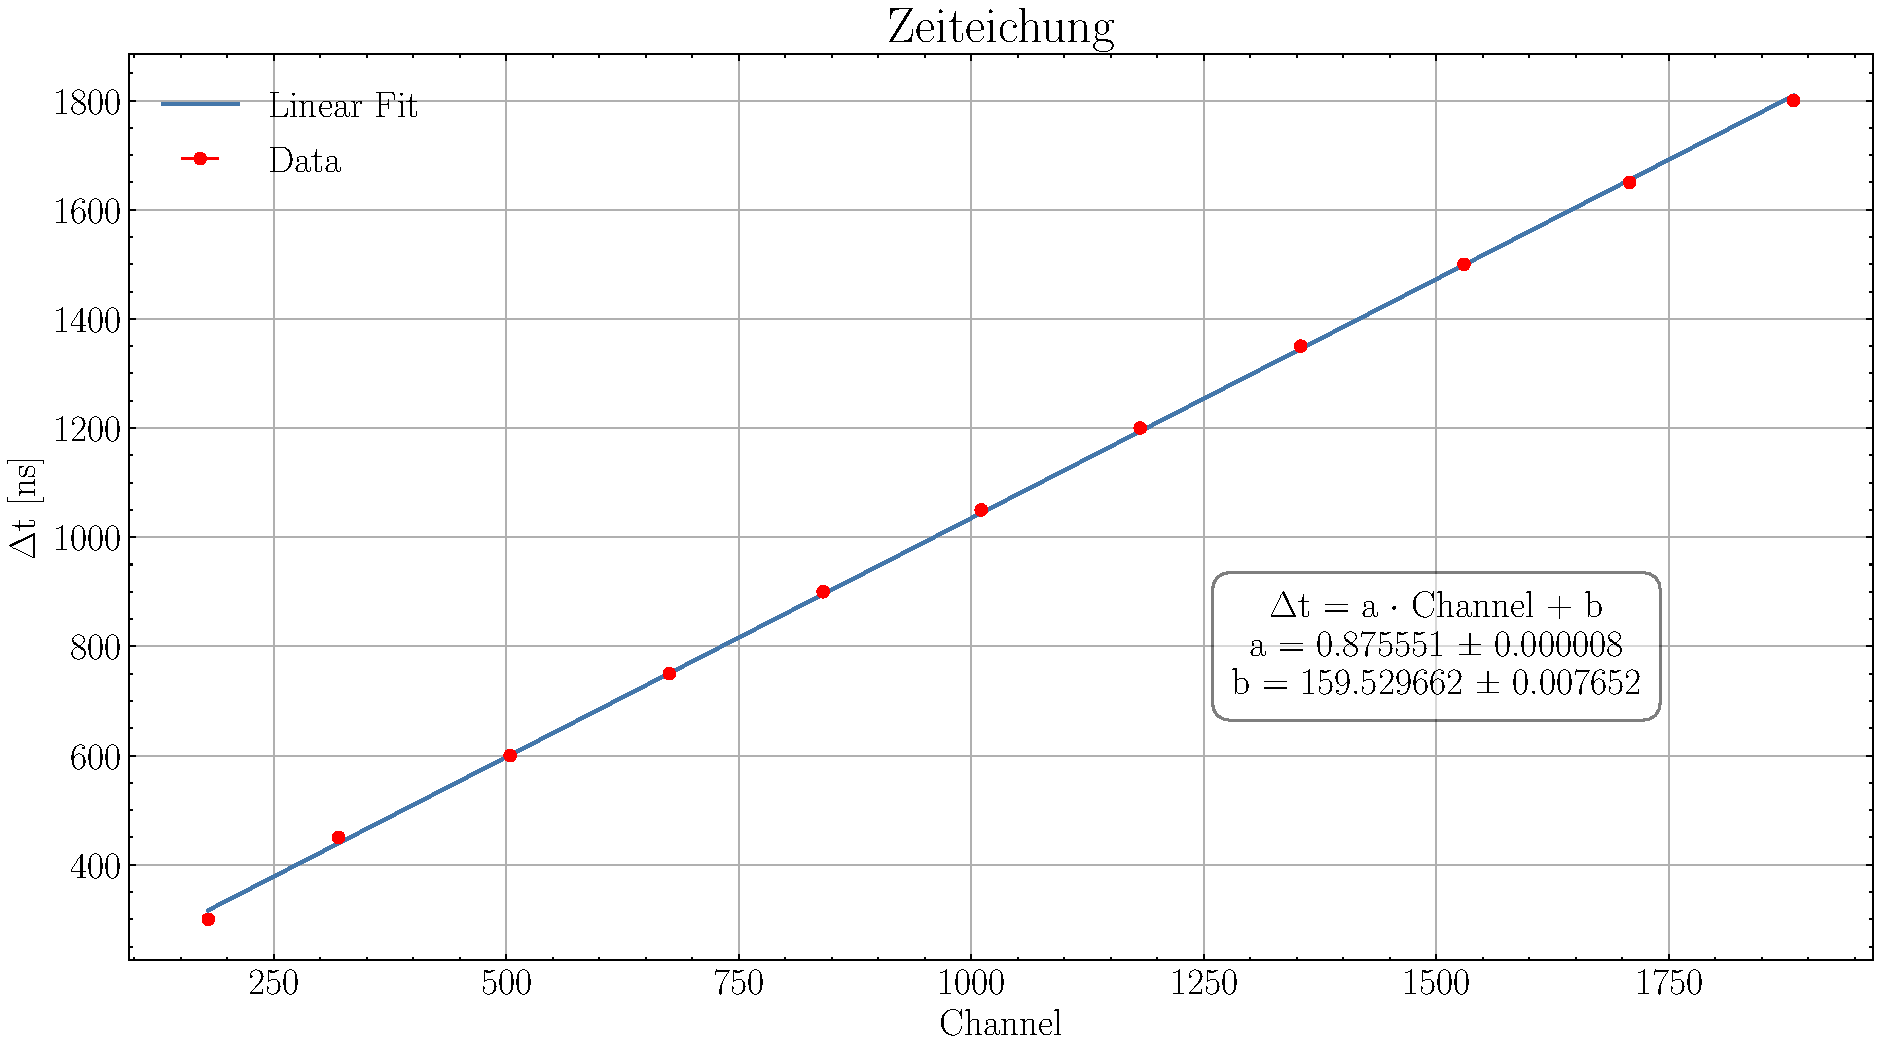
\includegraphics[width=\textwidth]{Bilder/timeLinearFit.pdf}		
		\caption{Gewichteter linearer Fit, der Kanallagen zu den Verzögerungen, wobei die Fehler der Kanallagen sehr klein sind und deshalb nicht im Plot erkennbar sind}
		\label{img:timeLinearFit}
	\end{figure}
	Damit besteht nun folgender Zusammenhang zwischen Zeitdifferenz $\Delta t$ und dem Kanal $K$:
	\begin{equation}
		\Delta t(K) = \SI{0.875551(0.000008)}{\nano \s} \cdot K + \SI{159.529662(0.007652)}{\nano \s}
	\end{equation}
	Die Fehler der Eichung sind sehr klein, was an der hohen Zahl von Eichpunkten liegen kann.

		
	\section{Lebensdauerbestimmung}
		\fehlt


\chapter{Fazit}

	\listoffigures
	% \addcontentsline{toc}{chapter}{\listfigurename}
	
	\begin{thebibliography}{111} %\addcontentsline{toc}{chapter}{Literaturverzeichnis}
		\bibitem{Anleitung}
		Dr. Hans Georg Zaunick, Stefan Diehl. \glqq Bestimmung der Lebensdauer von Myonen\grqq. Überarbeitete und aktualisierte Version. Aus: II. Physikalisches Institut
		Uni Gießen (2024).
		
		\bibitem{PDGLeptonen}
		Pdg. (2024) pdgLive. Retrieved June 24, 2024, from \url{https://pdglive.lbl.gov/Particle.action?node=S004&init=0}
		
		
		
	\end{thebibliography}


\chapter*{Anhang} \label{ch:Anhang}
\addcontentsline{toc}{chapter}{Anhang}
\FloatBarrier
	\begin{figure}[ht]
	\centering
	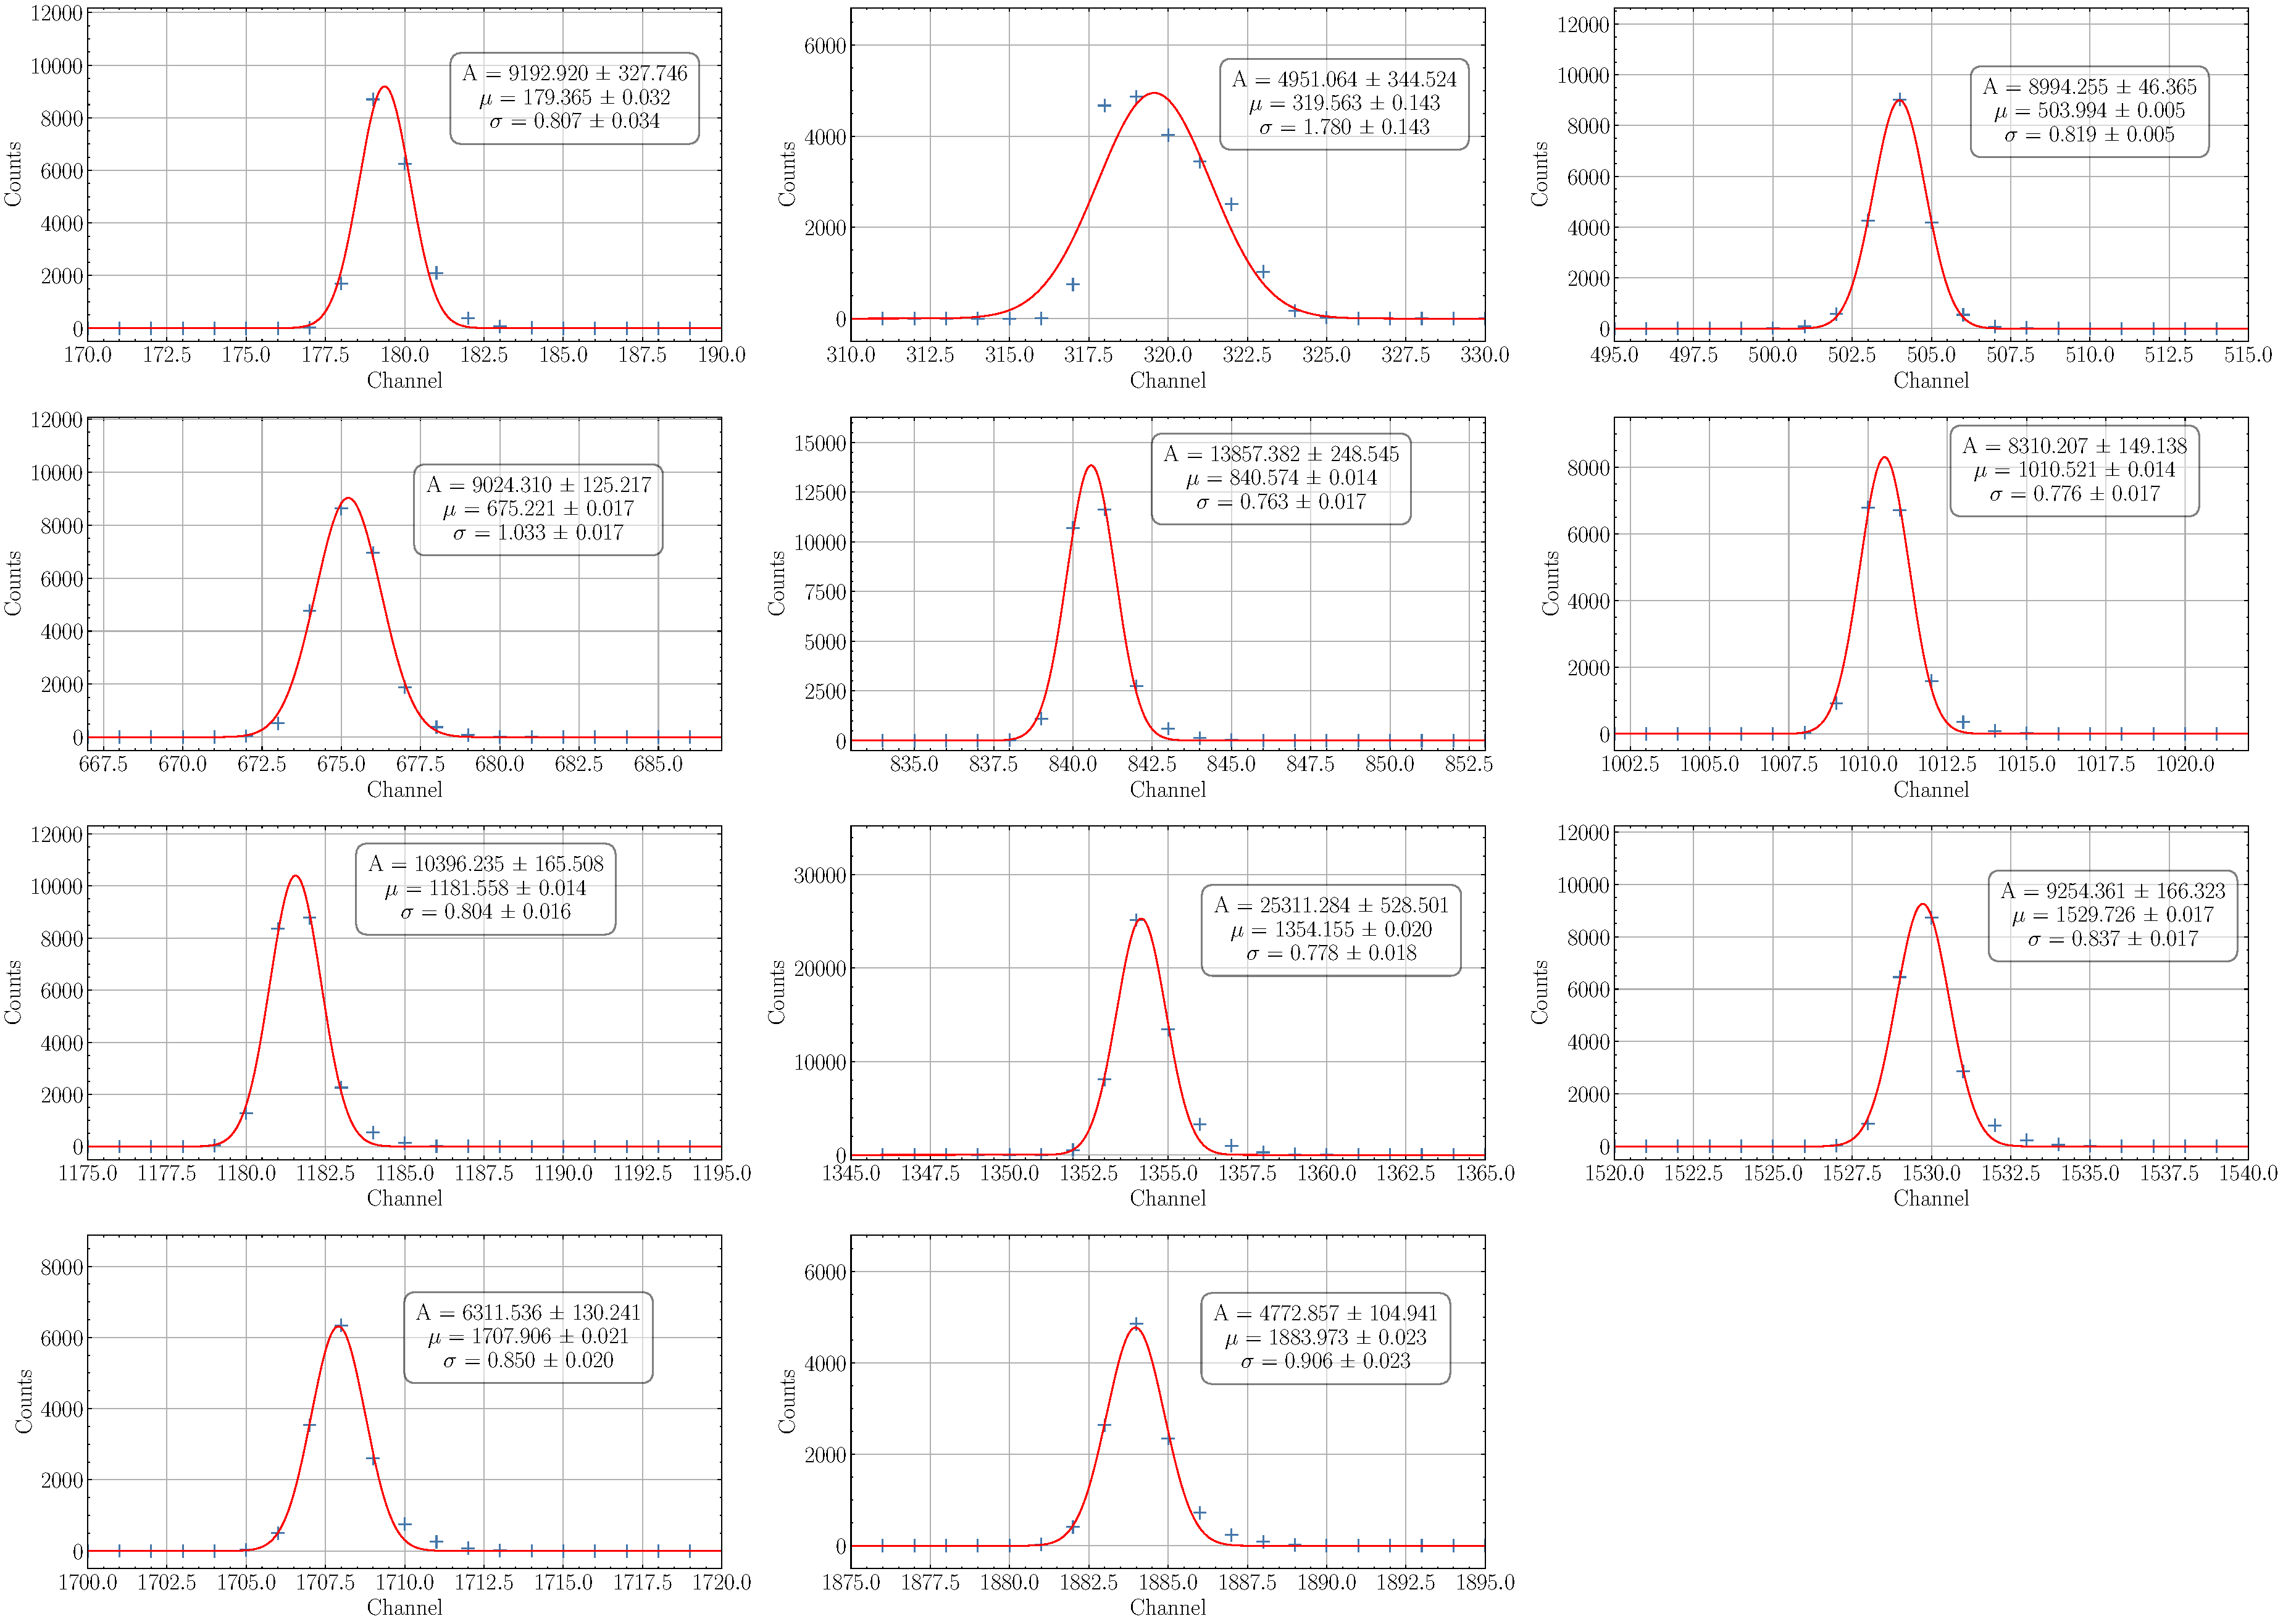
\includegraphics[width=\textwidth]{Bilder/timeGaussFits.pdf}		
	\caption{Gaußfits der einzelnen Zeitmessungen für die Zeiteichung}
	\label{img:TimeGauss}
\end{figure}





\end{document}
